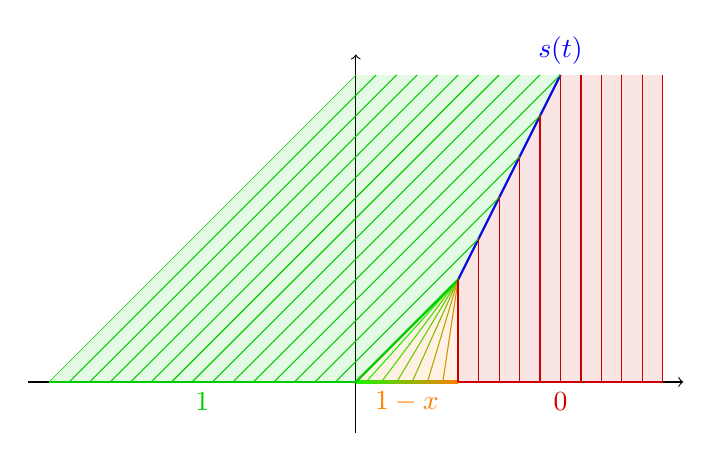
\begin{tikzpicture}[scale = 1.3]
\draw[thin, ->] (-3.2, 0) -- (3.2, 0);
\draw[thin, ->] (0, -0.5) -- (0, 3.2);

\draw[green!80!black, thick] (-3,0) -- node[midway, below] {$1$} (0,0);

\node[orange, below] at (0.5, 0) {$1-x$};
\draw[red!80!black, thick] (1,0) -- node[midway, below] {$0$} (3,0);

\draw[blue, thick] (1,1) -- (2, 3) node[above] {$s(t)$};

\begin{scope}
\clip (-3, 0) -- (0,3) -- (2,3) -- (1,1) -- (0,0) -- cycle;
\fill[green!80!black, opacity = 0.1] (-3,0) rectangle (3,3);
\foreach \p in {-3, -2.8, ..., 0}
	\draw[green!80!black] (\p, 0) -- ({\p + 3}, 3);
\end{scope}

\begin{scope}
\clip (0,0) -- (1,1) -- (1,0) -- cycle;
\fill[orange, opacity = 0.1] (0,0) rectangle (1,1);
\foreach \p in {0.1, 0.25, ..., 1} {
	\pgfmathsetmacro{\pctgblack}{int(100 * (\p))}
	\draw[{orange!\pctgblack!green}] (\p, 0) -- (1, 1);
}
\end{scope}
\fill[left color = orange!10!green, right color = orange!100!black] (0, -0.01) rectangle (1,0.01);

\begin{scope}
\clip (1,0) -- (1,1) -- (2,3) -- (3,3) -- (3,0) -- cycle;
\fill[red!80!black, opacity = 0.1] (1,0) rectangle (3,3);
\foreach \p in {1, 1.2, ..., 3}
	\draw[red!80!black] (\p, 0) -- (\p, 3);
\end{scope}

\draw[thick, green!80!black] (0,0) -- (1,1);
\draw[thick, red!80!black] (1,0) -- (1,1);

\end{tikzpicture}
